\documentclass[border=10pt]{standalone}

\usepackage[latin1]{inputenc}
\usepackage{tikz}
\usetikzlibrary{automata, positioning, arrows}
\begin{document}
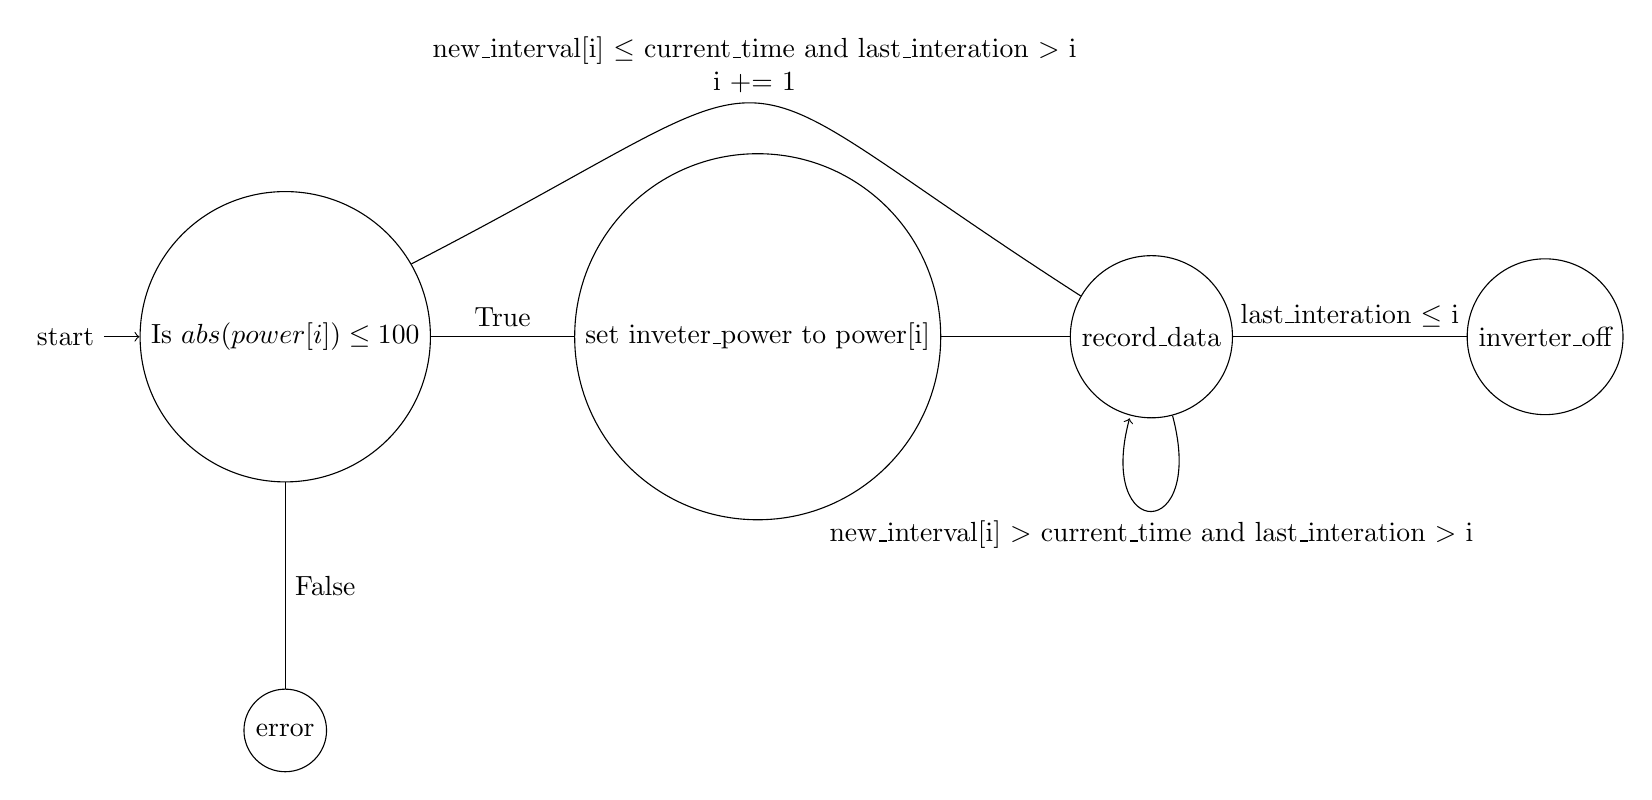
\begin{tikzpicture}
\node[state, initial] (q1) {Is $abs(power[i]) \leq 100$};
\node[state, right of=q1, xshift=5cm] (q2) {set inveter\_power to power[i]};
\node[state, right of=q2, xshift=4cm] (q3) {record\_data};
\node[state, right of=q3, xshift=4cm] (q4) {inverter\_off};
\node[state, below of=q1, yshift=-4cm] (q5) {error};

\draw 
(q1) edge[above] node{True} (q2)
(q1) edge[right] node{False} (q5)
(q2) edge[above] node{} (q3)
(q3) edge[loop below] node{new\_interval[i] $>$ current\_time and last\_interation $>$ i} (q3)
(q3) edge[above] node{last\_interation $\leq$ i} (q4)
(q3) edge[bend right, above, min distance=6cm] node[align = center] {new\_interval[i] $\leq$ current\_time and last\_interation $>$ i \\ i += 1} (q1);
\end{tikzpicture}
\end{document}